\section{Inverse Trigonometric Functions}
We will now show how a Gauss--Legendre quadrature approach can also be used for efficient privacy-preserving approximation of the inverse tangent function. Two well-known series representations of the arctangent function exist: the Maclaurin series expansion,
\begin{align} \label{eq:arctan_maclaurin}
	\arctan x = \sum_{n=0}^{\infty}{\frac{(-1)^nx^{2n+1}}{2n+1}}, \text{ for }|x|\leq 1
\end{align}
and the following series expansion discovered by Euler in 1755, which converges more rapidly for all $x$~\cite{chien-lih_89.67_2005}.
\begin{align} \label{eq:arctan_euler}
	\arctan x = \sum_{n=0}^{\infty}
	{
	\frac
		{2^{2n}(n!)^2}
		{(2n+1)!}
	\frac
		{x^{2n+1}}
		{(1+x^2)^{n+1}}
	}
\end{align}
We will compare the quadrature approach with the method of computing partial sums from each of these series.

To obtain a Gauss--Legendre quadrature-based approximation, we take the following integral,
\begin{align*}
	\arctan x = \int_0^x{\frac{1}{1+x^2}\diff x},
\end{align*}
and perform five-point Gauss--Legendre quadrature to obtain the following closed-form approximation:
\begin{align} \label{eq:arctan_quadrature}
	\begin{split}
		&\arctan x \\
		&= \frac
		{4\left(225x^9 + 15925x^7 + 144753x^5 + 350595x^3 + 238140x\right)}
		{15\left(x^{10} + 480x^8 + 11760x^6 + 64120x^4 + 114660x^2 + 63504\right)}
	\end{split}
\end{align}

We note that in order to evaluate the quadrature approximation in Equation~\ref{eq:arctan_quadrature}, we must compute the value of $x^{10}$, which requires several rounds of the squaring and multiplication protocols to compute. We now compare the quadrature approximation to the partial sum composed of the first 4 terms of Euler's series expansion in Equation~\ref{eq:arctan_euler}, which requires a similar number of floating-point operations to compute:
\begin{align} \label{eq:arctan_euler_partial}
	\begin{split}
		&\sum_{n=0}^{3}
		{
		\frac
			{2^{2n}(n!)^2}
			{(2n+1)!}
		\frac
			{x^{2n+1}}
			{(1+x^2)^{n+1}}
		}\\
		&= \frac
		{965x^9 + 2370x^7 + 2688x^5 + 1470x^3 + 315x}
		{315\left(x^{10} + 5x^8 + 10x^6 + 10x^4 + 5x^2 + 1\right)}
	\end{split}
\end{align}

Figure~\ref{fig:arctan_error} shows that despite requiring a similar number of floating-point operations, the quadrature based approximation in Equation~\ref{eq:arctan_quadrature} gives accurate approximations over a larger interval, making it a more viable candidate for efficient computation.
\begin{figure}[!ht]
		\centering
		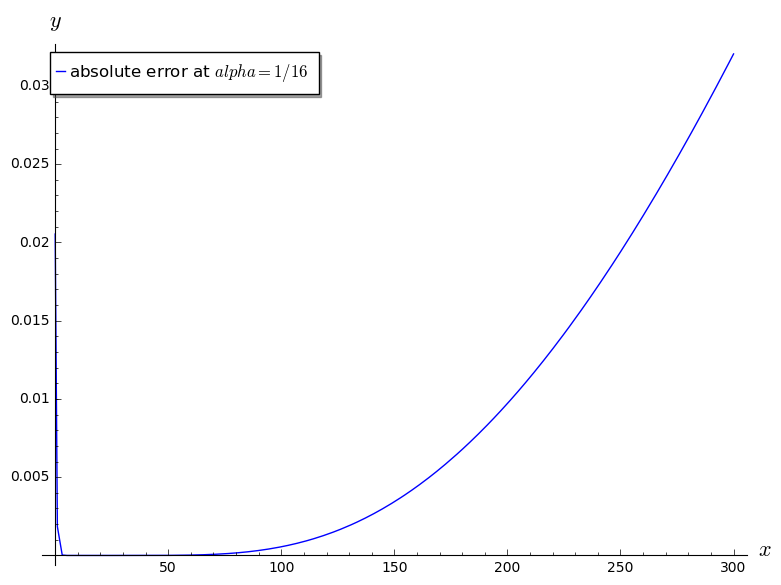
\includegraphics[width=.9\linewidth]{figures/single_alpha_plot.png}
		\caption{Comparison of the absolute error of the approximations for $\arctan x$ using quadrature approximation (Equation~\ref{eq:arctan_quadrature}) and the first 4 terms of Euler's series (Equation~\ref{eq:arctan_euler_partial})}
		\label{fig:arctan_error}
\end{figure}

Figure~\ref{fig:arctan_error_2} shows the absolute error of the quadrature approximation over the interval $[-1,1]$. Since the quadrature approximation yields results with high accuracy over this interval, potential implmentations may use the following trigonometric identities to calculate values of the inverse tangent at larger arguments.
\begin{align*}
	\arctan x =
	\begin{cases}
		\frac{\pi}{2}-\arctan{\frac{1}{x}} & \text{if } x > 0 \\
		-\frac{\pi}{2}-\arctan{\frac{1}{x}} & \text{if } x < 0 
	\end{cases}
\end{align*}

To carry out the conditional check required to use these identities, a privacy-preserving comparison protocol may be used, such as in~\cite{veugen_improving_2012}.
\begin{figure}[!ht]
		\centering
		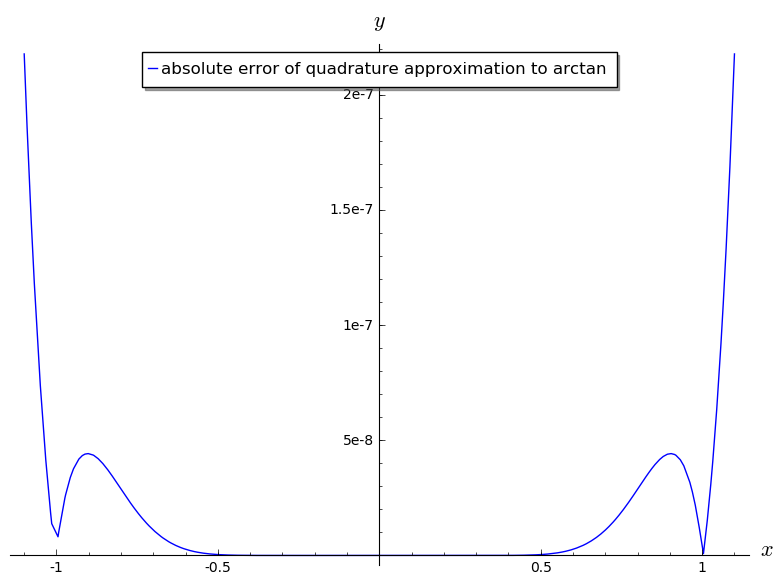
\includegraphics[width=.9\linewidth]{figures/arctan_error_2.png}
		\caption{Absolute error of the approximation for $\arctan x$ using quadrature approximation (Equation~\ref{eq:arctan_quadrature}) over the interval $[-1,1]$}
		\label{fig:arctan_error_2}
\end{figure}
